It follows from Lemma \ref{maxmin} that in order to approximate a continuous function $f: K \to \bb{R}^m$ using a ReLU net, it suffices to approximate $f$ with a max-min string. The goal of section \ref{main} below is to show how this can be done. The proof will require some technical analysis, but the broad idea is highlighted well by considering the case when $K$ is a finite set. In fact, in the finite case, $f$ can be computed exactly using a ReLU net:
\begin{lemma}
\label{finitecase}
Let $\epsilon \in \bb{R}_{>0}$ and $f: S \to \bb{R}^m$ a function with $S$ finite. Then there exists a max-min string $g: \bb{R}^n \to \bb{R}^m$ such that $f = g$.
\end{lemma}
The following Lemma will be used:
\begin{lemma}
\label{bigaffinefunctionfinite}
Let $f: S \to \bb{R}^m$ be a function with $S \subseteq \bb{R}^n$ a finite set. For any $t \in \bb{R}_{\geq 0}$ and any $x \in \bb{R}\setminus S$ there exists an affine function $l = (l_1,...,l_m): \bb{R}^n \to \bb{R}^m$ such that
\begin{itemize}
    \item $l(x) = (0,...,0)$,
    \item $t < l_i(s)$ for all $s \in S$
\end{itemize}
\end{lemma}
\begin{proof}
Many such functions $l$ can be defined, but in order to reflect the construction which will be used to prove the case where $S$ is an arbitrary compact set, the case when $n = 2$ and $m = 1$ will be considered and a particular construction will be shown which perhaps is not the most obvious one.\\\\
%
Let $A,B \in \bb{R}^2$ be points such that $\Delta AxB$ forms a triangle, $S\cap \Delta AxB = \lbrace x \rbrace$ and $S$ lies in the infinite planar sector $\angle AxB$, ie
\[S \subseteq \angle AxB := \lbrace \big(\gamma_1(B - x),\gamma_2(C - x)\big) \mid \gamma_1,\gamma_2 \geq 0\rbrace\]
see figure \ref{infiniteplanarsector}.
\begin{figure}
    \centering
    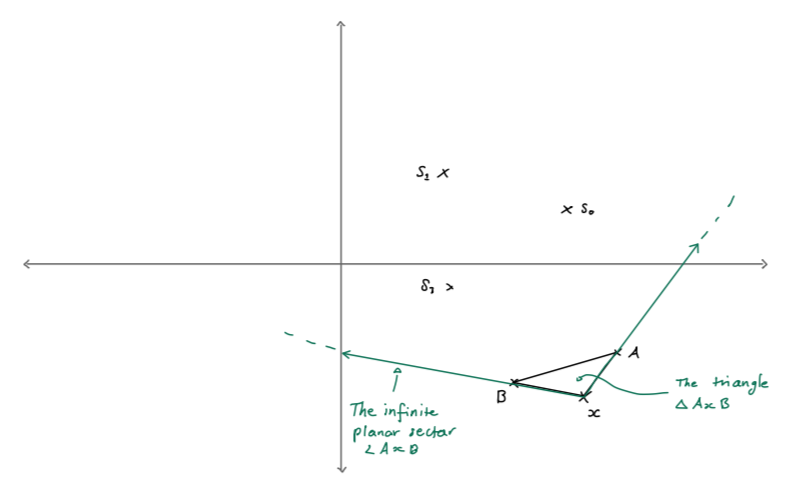
\includegraphics[width = \textwidth]{Sections/Diagrams/infiniteplanarsector.png}
    \caption{An example of an appropriate choice of triangle for the proof of Lemma \ref{bigaffinefunctionfinite}.}
    \label{infiniteplanarsector}
\end{figure}
Then let $l$ be the affine function such that $l(x) = 0$ and $l(A) = l(B) = t$. See figure \ref{bigaffinefinitezero}
\begin{figure}
    \centering
    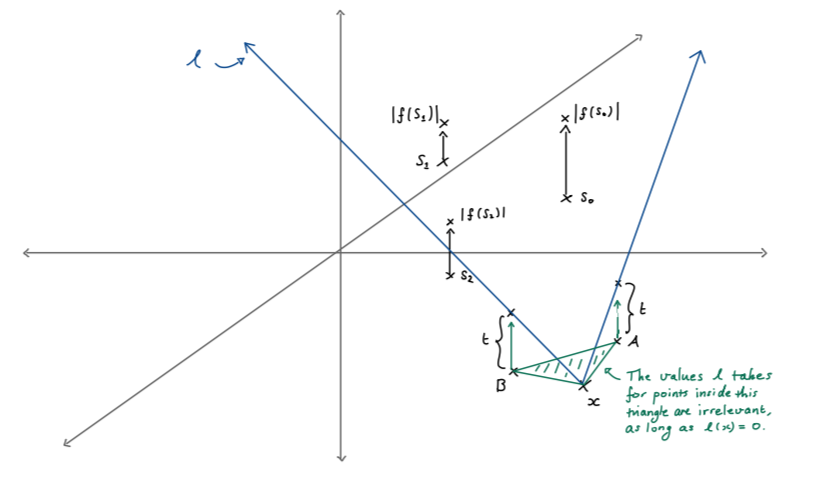
\includegraphics[width=\textwidth]{Sections/Diagrams/bigaffinefinite.png}
    \caption{The affine function $l$.}
    \label{bigaffinefinitezero}
\end{figure}
\end{proof}
%
\begin{proof}[Proof of Lemma \ref{finitecase}]
If $S = \lbrace s \rbrace$ contains a single element, then the max-min string $g(s) = f(s)$ can be used. So say $S$ contains at least two elements. Fix an element $s \in S$ and let $g: S\setminus\lbrace s \rbrace \to \bb{R}^m$ be a max-min string satisfying $\forall s' \in S\setminus\lbrace s\rbrace$, $g(s') = f(s')$. Set 
\[t = \operatorname{max}_{s' \in S \setminus \lbrace s \rbrace}\lbrace |g(s') - f(s)|\rbrace\]
and let $l = (l_1,...,l_m): \bb{R}^n \to \bb{R}^m$ be an affine function such that $l(s) = 0$ and for all $s' \in S \setminus \lbrace s \rbrace$, $l_i(s') > t$, which exists by Lemma \ref{bigaffinefunctionfinite}. Write $f = (f_1,...,f_m)$, then 
\begin{equation}
\label{lboundfinite}
\forall s' \in S\setminus\lbrace s \rbrace,\forall i = 1,...,m,\qquad f_i(s) - l_i(s') < g_i(s') < f_i(s) + l_i(s')
\end{equation}
Define the max-min string:
\[\hat{g} = \operatorname{max}\lbrace \operatorname{min}\lbrace g, f(s) + l\rbrace, f(s) - l\rbrace\]
which is such that $\hat{g}(s') = f(s')$ for all $s' \in S$. Indeed,
\begin{align*}
    \hat{g}(s) &= \operatorname{max}\lbrace \operatorname{min}\lbrace g(s), f(s) + l(s)\rbrace, f(s) - l(s)\rbrace\\
    &= \operatorname{max}\lbrace \operatorname{min}\lbrace g(s), f(s)\rbrace, f(s)\rbrace\\
    &= f(s)
\end{align*}
and if $s' \in S\setminus \lbrace s \rbrace$,
\begin{align*}
    \hat{g}(s') &= \operatorname{max}\lbrace \operatorname{min}\lbrace g(s'), f(s) + l(s')\rbrace, f(s) - l(s')\rbrace\\
    &= \operatorname{max}\lbrace g(s'), f(s) - l(s')\rbrace\\
    &= g(s') = f(s')
\end{align*}
where the first and second equality follow from \ref{lboundfinite}.
\end{proof}